\documentclass[a4paper,12pt]{article} 



%Добавляет возможность искать и копировать текст
\usepackage{cmap}

%Убирает пробел между названием таблицы/рисунка и самой таблицей/рисунком
\usepackage{caption}
\captionsetup[table]{skip= -0 cm}
\captionsetup[figure]{skip= -0 cm}

%Выравнивание названия таблиц по левому краю
%\usepackage[nooneline]{caption} 
%Размеры отступов 
\usepackage[left=20mm, top=20mm, right=20mm, bottom=20mm, footskip=10mm]{geometry}

%Рисунки
\usepackage{graphicx}
\usepackage{wrapfig} %обтекание элементов
\graphicspath{{graphs}{figures}}  % папки с картинками

%Русский язык в формулах
\usepackage{mathtext}

%  Русский язык
\usepackage[T2A]{fontenc}			
\usepackage[utf8]{inputenc}			
\usepackage[english,russian]{babel}	

%Готические буквы
\usepackage{amssymb}

% Математика
\usepackage{amsmath,amsfonts,amssymb,amsthm,mathtools} 
\usepackage{wasysym}

%Цветные подписи в таблице
\usepackage[table,xcdraw]{xcolor}

\usepackage{fancyhdr} % Колонтитулы
 	\pagestyle{fancy}
 	\renewcommand{\headrulewidth}{0.3mm}  % Толщина линейки, отчеркивающей верхний колонтитул
 	%\lfoot{Нижний левый}
 	%\rfoot{Нижний правый}
 	\rhead{Белостоцкий Артмемий, Б04-006}
 	%\chead{Верхний в центре}
 	\lhead{Лабораторная работа №4.5.2}
 	% \cfoot{Нижний в центре} % По умолчанию здесь номер страницы
 	
 	
\begin{document} 

%Титульник 
\begin{titlepage}
	\begin{center}
		\large 	МИНИСТЕРСТВО ОБРАЗОВАНИЯ И НАУКИ РОССИЙСКОЙ ФЕДЕРАЦИИ\\
				МОСКОВСКИЙ ФИЗИКО-ТЕХНИЧЕСКИЙ ИНСТИТУТ \\
				(НАЦИОНАЛЬНЫЙ ИССЛЕДОВАТЕЛЬСКИЙ ИНСТИТУТ)\\ 
				ФИЗТЕХ-ШКОЛА ЭЛЕКТРОНИКИ, ФОТОНИКИ \\
				И МОЛЕКУЛЯРНОЙ ФИЗИКИ \\
		
		
		\vspace{4.0 cm}
		Лабораторная работа № 4.5.2 \\ 
		\LARGE \textbf{Интерференция лазерного излучения}
	\end{center}
	\vspace{3 cm} \large
	
	\begin{flushright}
		выполнил студент 2 курса \\
		{группы Б04-006}\\
		\textbf{Белостоцкий Артемий}\\
	\end{flushright}
	
	\vfill

	\begin{center}
	Долгопрудный, 2022 г.
	\end{center}
\end{titlepage}                                                                      

\section*{Цель работы}
Исследовать зависимость видности интерференционной картины от разности хода интерферирующих лучей и от их поляризации

\section*{В работе используются}
\begin{itemize}
\item Не-Nе лазер
\item интерферометр Майкельсона
\item с подвижным зеркалом 
\item фотодиод с усилителем 
\item осциллограф С1-76
\item поляроид
\item линейка
\end{itemize}

\section*{Теоретические сведения}

Для описания чёткости интерференционной
картины в некоторой
точке Майкельсон ввёл параметр видности $\gamma$:
\begin{equation}
\gamma = \frac{I_{max}-I_{min}}{I_{max}-I_{min}}
\end{equation}

где $I_{max}$ и  $I_{min}$ - максимальная и минимальная интенсивности света интерфереционной картины вблизи выбранной точки. Параметр $\gamma$ меняется в пределах от 0 (полное исчезновение интерфереционной картины) до 1(наиболее четкая картина). Человеческий глах может уверенно различать чередование светлых и темных интерфереционных полос,если $\gamma > 0,1$

Пусть в плоскости наблюдения интерферируют по
д небольшим углом две волны с амплитудами $A_m$ и $B_m$.Если в точке наблюдения разность фаз между волнами равна $k_m l$, где $k_m =2 \pi / \lambda_m$, l - разность хода, тогда интенсивность света в данной точке:

\begin{equation}
I_m = A_m^2 + B_m^2 + 2 A_m B_m cos(k_m l)
\end{equation}

При этом интенсивность свет
а в максимуме интерференционной
картины $I_{max} = (A_m + B_m)^2$, а в минимуме $I_{min} = (A_m - B_m)^2$

видность 

\begin{equation} \label{eq:gamma_1}
\gamma_1 = \frac{2 \sqrt{\delta}}{1 + \delta}
\end{equation}

где параметр 

\begin{equation}
\delta = \frac{B_m^2}{A_m^2}
\end{equation}

выражает отношение интенсивностей интерферирующих волн.

Учитывая спектральный состав света, видность интерфереционной картины:

\begin{equation}
\gamma = \gamma_1 \gamma_2(l)
\end{equation}

где 

\begin{equation}
\gamma_2 = \frac{\sum\limits_{n}A_n^2 \cos \left(\frac{2 \pi \delta \nu n l}{c}\right)}{\sum\limits_{n}A_n^2} \approx e^{-(\pi \Delta F l/c)^2}
\end{equation}

Таким образом

\begin{equation} 
\label{eq:halfWidth}
l_{1/2} = \frac{0,26c}{\Delta F}
\end{equation}

\begin{figure}[h]
	\begin{center}
	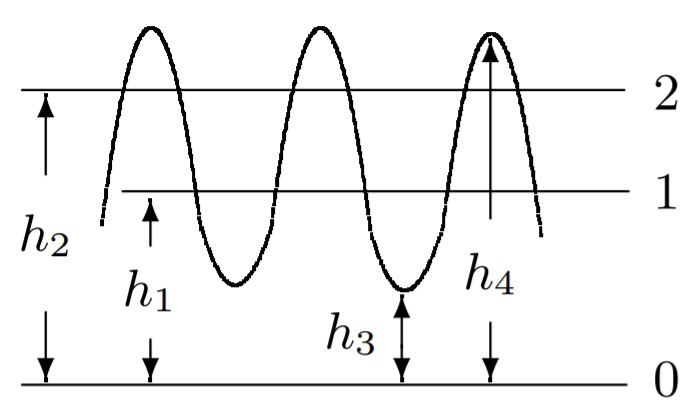
\includegraphics[scale=0.3]{fig1}
	\label{fig:setup}
	\caption{Схема экспериментальной установки}
	\end{center}
\end{figure}

Осциллограф используетс
я для регистрации следующих сигналов: фоновой засветки (линия 0 — перекрыты оба луча 1 и 2); интенсивности свет а одного из пучков (линии 1 или 2
— перекрыт луч 2 или 1); максимума
и минимума интенсивности интерференционной
картины (открыты оба луча). При этом параметр $\delta$ определяется отношением:

\begin{equation} 
\label{eq:delta}
\delta = \frac{h_1}{h_2}
\end{equation}

Видность интерференционной
картины рассчитывается
я по формуле:

\begin{equation}
\label{eq:gamma}
\gamma = \frac{h_4 - h_3}{h_4 + h_3}
\end{equation}

При $\alpha = 0 (\gamma_3 = 1)$:

\begin{equation}
\label{eq:gamma_2}
\gamma_2(l) = \frac{\gamma}{\gamma_1}
\end{equation}

При l = 0 ($\gamma_2 = 1$):
\begin{equation}
\label{eq:gamma_3}
\gamma_3 = \frac{\gamma}{\gamma_1}
\end{equation}

\newpage

\section*{Экспериментальная установка}

\begin{figure}[h]
	\begin{center}
	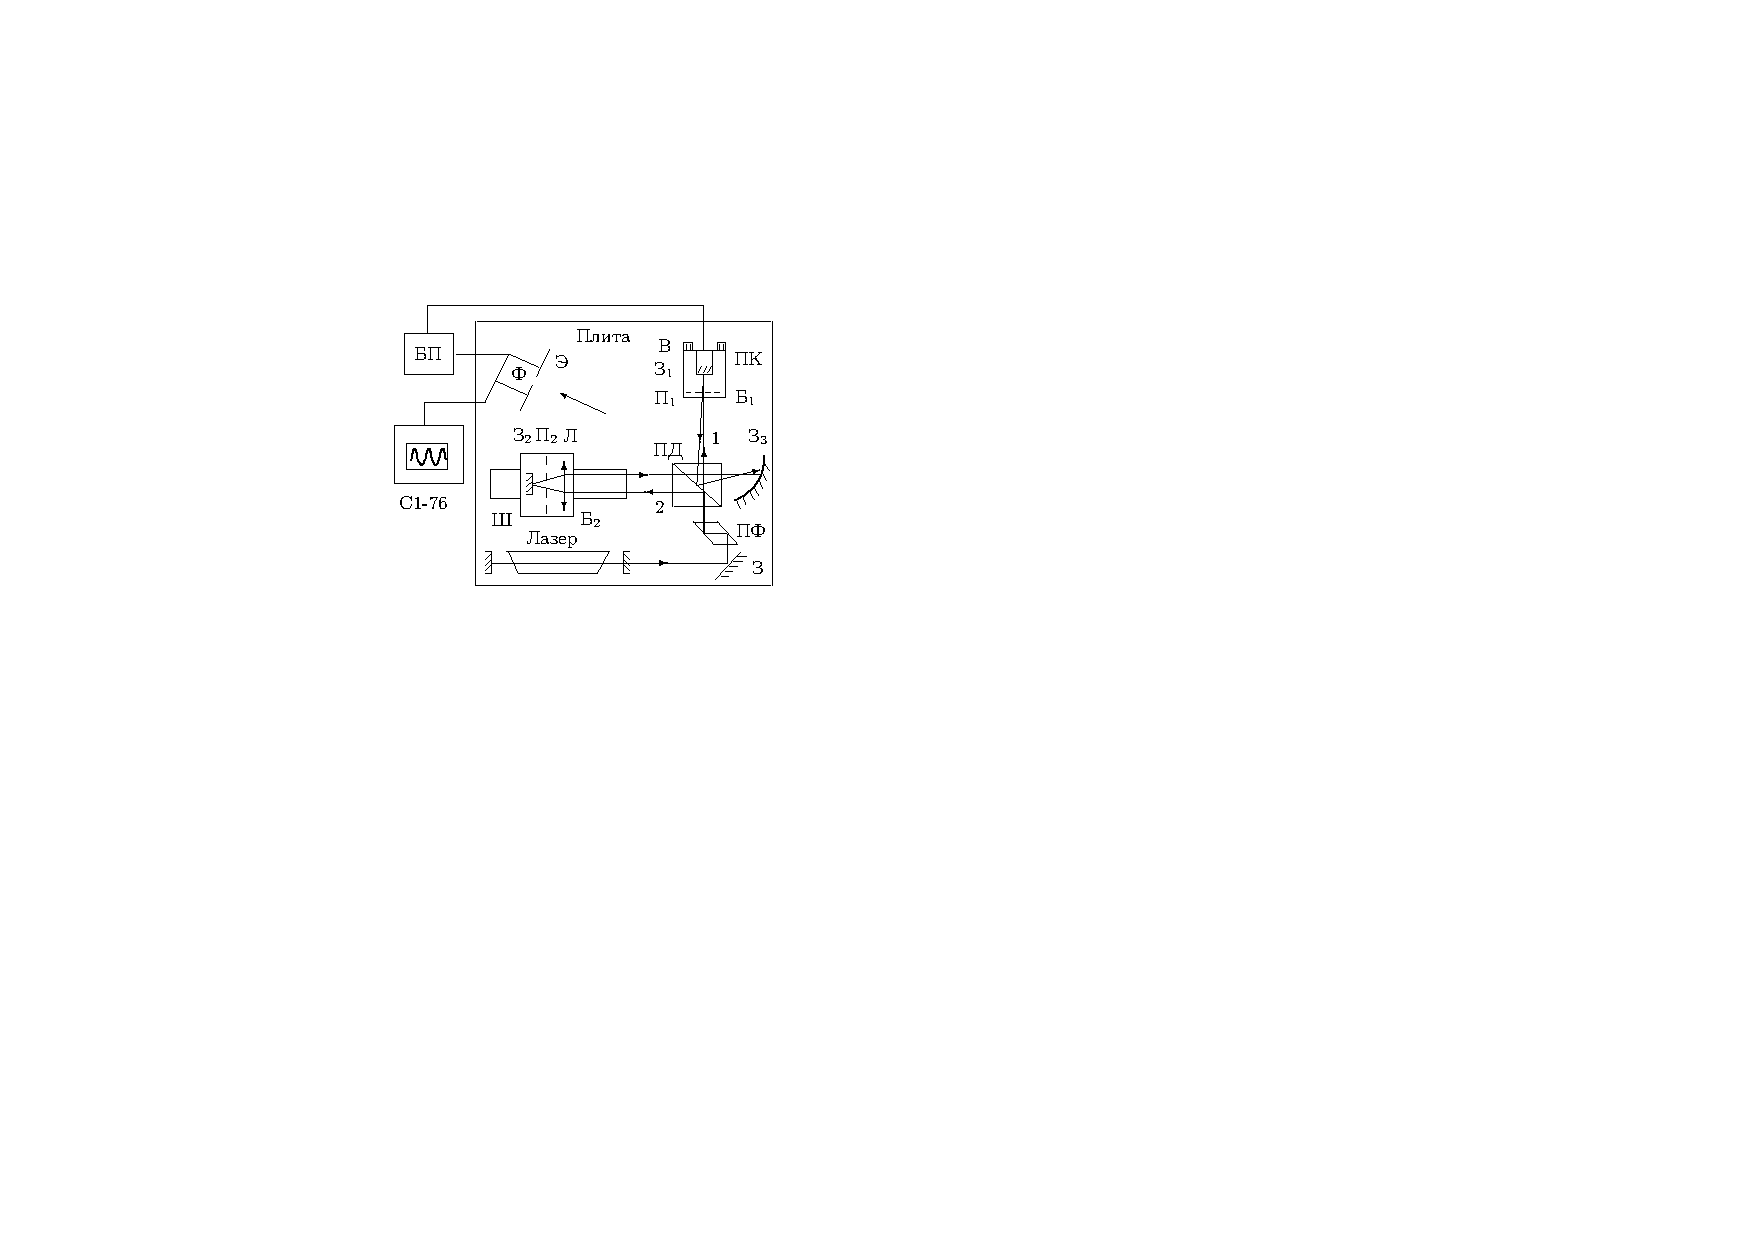
\includegraphics[scale=1.5]{setup}
	\label{fig:setup}
	\caption{Осциллограмма сигналов фотодиода}
	\end{center}
\end{figure}

	Луч 1 проходит поляроид $П_1$, отражается под небольшим углом от зеркала $З_1$, снова проходит
	поляроид $П$ и, частично отражаясь от диагональной плоскости делительной призмы, выходит из интерферометра. Зеркало $З_1$ наклеено на пьезокерамику ПК, которая может осуществлять малые
	колебания зеркала вдоль падающего луча. Поляроид и зеркало с пьезокерамикой собраны в единый блок $Б_1$, который крепится к вертикально стоящей плите. В блоке $Б_1$ имеются юстировочные винты В, которые позволяют регулировать угол наклона зеркала $З_1$ В установке предусмотрена возможность вращения поляроида $П_1$ вокруг луча 1. Угол поворота отсчитывается по шкале, нанесённой на оправу поляроида.
	
	Луч 2 проходит линзу Л, поляроид $П_2$, отражается от зеркала $З_2$, снова проходит поляроид $П_2$, линзу Л и частично выводится делительной призмой из интерферометра. Зеркало $З_2$ установлено в фокальной плоскости линзы Л. Это сделано для того, чтобы падающий и выходящий из системы лучи всегда были параллельны друг другу. Линза Л, поляроид $П_2$ и зеркало $З_2$ собраны в единый блок $Б_2$. Этот блок может перемещаться вдоль луча 2 по штанге Ш, жёстко связанной с плитой интерферометра. Длина штанги 90 см. В установке предусмотрена возможность небольшого перемещения блока $Б_2$ перпендикулярно лучу, что позволяет регулировать расстояние между падающим и выходящим из блока лучами. При измерениях блок $Б_2$ крепится к штанге при помощи двух винтов. Вдоль штанги нанесены деления через один сантиметр. При перемещении блока $Б_2$ вдоль штанги на величину $ l_1 $ геометрическая разность хода между лучами 1 и 2 изменяется на величину $ l = 2l_1 $.
	
	Лучи 1 и 2 накладываются друг на друга и интерферируют вблизи задней грани делительной призмы ПД. Сферическое зеркало $З_3$ с небольшим фокусным расстоянием увеличивает картину интерференционных полос и проецирует её на экран Э.
	
\newpage

\section*{Ход работы}

\subsection*{Измерение коэффициента видности}

Исследуем зависимость видности интерфереционной картины от угла поворота поляроида $\alpha$. Для этого будем измерять величины $h_1,h_2, h_3, h_4$. Полученные данные занесем в Таблицу $\ref{table:alpha}$

\begin{table}[h]
\begin{center}
\caption{}
\label{table:alpha}
\begin{tabular}{|c|c|c|c|c|}
\hline 
$\alpha$,$^\circ $  & h1, дел & h2, дел & h3, дел & h4, дел \\ \hline
10                     & 4                         & 4                         & 3                & 12               \\ \hline
20                     & 3,5                       & 3,5                       & 3                & 11,5             \\ \hline
30                     & 4                         & 3,5                       & 3                & 11               \\ \hline
40                     & 6                         & 3                         & 5                & 13               \\ \hline
50                     & 5                         & 2,5                       & 4,5              & 10,5             \\ \hline
60                     & 6,5                       & 2                         & 6                & 11               \\ \hline
70                     & 5                         & 2                         & 5                & 8,5              \\ \hline
80                     & 4,5                       & 2                         & 5                & 7                \\ \hline
90                     & 4                         & 1,5                       & 5                & 6                \\ \hline
\end{tabular}
\end{center}
\end{table}

Рассчитаем коэффициент $\gamma_3$, используя формулы ($\ref{eq:gamma_1}$), ($\ref{eq:delta}$), ($\ref{eq:gamma}$), ($\ref{eq:gamma_3}$)

Оценим погрешности рассчитанных величин, учтя что $\sigma_h$ = 0,5 дел:

$$
\sigma_{\delta} = \delta \sqrt{ {\left(\frac{\sigma_h}{h_1}\right)}^2 + {\left(\frac{\sigma_h}{h_2}\right)}^2}	
$$

$$
\sigma_{\gamma_1} = 	\left( \frac{1}{\sqrt{\delta}(\delta + 1)} + \frac{\sqrt{\delta}}{(\delta + 1)^2} \right)  \sigma_{\delta}
$$

$$
\sigma_{\gamma} = \gamma \sqrt{ {\left(\frac{\sqrt{2}\sigma_h}{h_3 + h_4}\right)}^2 + {\left(\frac{\sqrt{2}\sigma_h}{h_3 - h_4}\right)}^2}	
$$

$$
\sigma_{\gamma_3} = \gamma_3 \sqrt{ {\left(\frac{\sigma_{\gamma_1}}{\gamma_1} \right)}^2 + {\left(\frac{\sigma_{\gamma}}{\gamma}\right)}^2}
$$


Полученные данные занесем в Таблицу $\ref{table:gamma_3}$

\newpage

\begin{table}[h!]
\label{table:gamma_3}
\caption{}
\begin{center}
\begin{tabular}{|c|c|c|c|c|c|c|c|c|c|}
\hline
cos($\alpha)$ & $cos(\alpha)^2$ & $\delta$     & $\sigma_{\delta}$  & $\gamma_1$    & $\sigma_{\gamma_1}$ & $\gamma_3$    & $\sigma_{\gamma_3}$ & $\gamma$    & $\sigma_{\gamma}$  \\ \hline
0,985 & 0,970  & 1,000 & 0,177 & 1,000 & 0,133 & 0,600 & 0,156 & 0,600 & 0,146 \\ \hline
0,940 & 0,883  & 1,000 & 0,202 & 1,000 & 0,152 & 0,586 & 0,156 & 0,586 & 0,143 \\ \hline
0,866 & 0,750  & 1,143 & 0,217 & 0,998 & 0,145 & 0,573 & 0,152 & 0,571 & 0,140 \\ \hline
0,766 & 0,587  & 2,000 & 0,373 & 0,943 & 0,146 & 0,471 & 0,083 & 0,444 & 0,067 \\ \hline
0,643 & 0,413  & 2,000 & 0,447 & 0,943 & 0,176 & 0,424 & 0,087 & 0,400 & 0,068 \\ \hline
0,500 & 0,250  & 3,250 & 0,850 & 0,848 & 0,196 & 0,347 & 0,065 & 0,294 & 0,039 \\ \hline
0,342 & 0,117  & 2,500 & 0,673 & 0,904 & 0,209 & 0,287 & 0,062 & 0,259 & 0,043 \\ \hline
0,174 & 0,030  & 2,250 & 0,616 & 0,923 & 0,214 & 0,181 & 0,041 & 0,167 & 0,029 \\ \hline
0,000 & 0,000  & 2,667 & 0,949 & 0,891 & 0,274 & 0,102 & 0,028 & 0,091 & 0,017 \\ \hline
\end{tabular}
\end{center}
\end{table}

Построим график зависимости $\gamma_3(\cos^2(\alpha))$ по данным Таблицы $\ref{table:gamma_3}$

\begin{figure}[h!]
	\begin{center}
	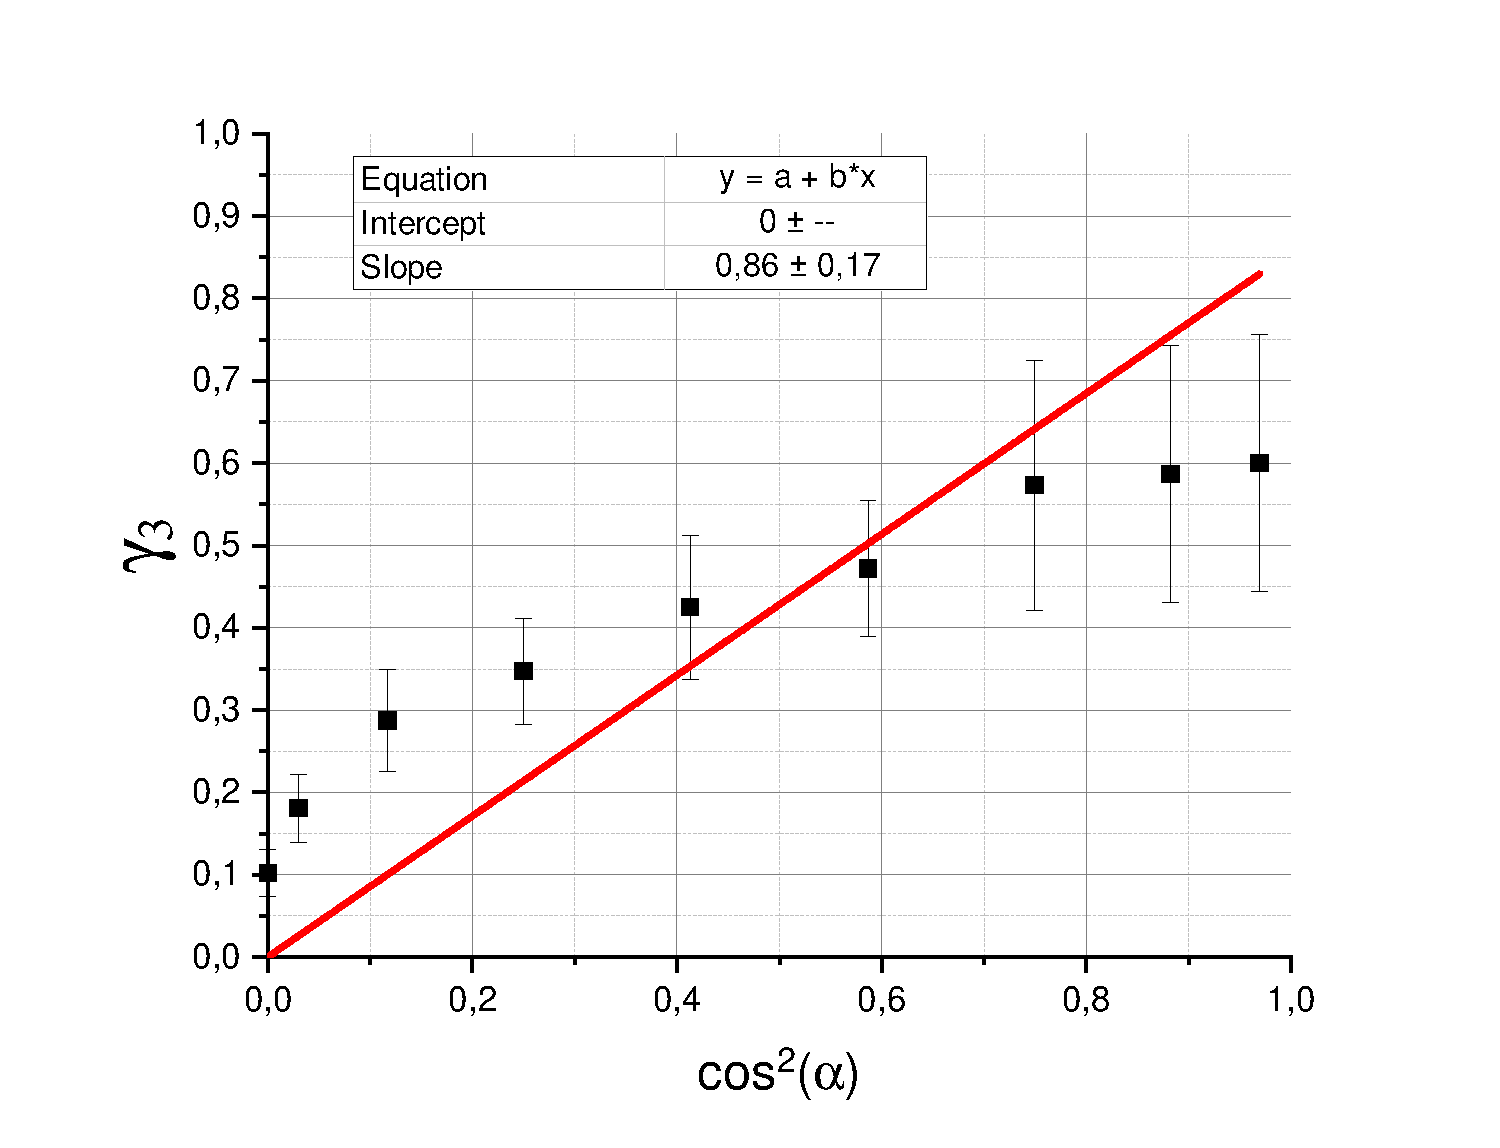
\includegraphics[scale=0.7]{graph1}
	\label{fig:graph1}
	\caption{График зависимости $\gamma_3(\cos^2(\alpha))$}
	\end{center}
\end{figure}

Исследуем зависимость видности от разности хода между лучами. Снимем зависимость величин $h_1, h_2, h_3, h_4$ от координаты x блока. Данные занесем в Таблицу 

\newpage

\begin{table}[h!]
\label{table:gamma_2}
\caption{}
\begin{center}
\begin{tabular}{|c|c|c|c|c|c|c|c|c|c|c|c|c|}
\hline
x  & $h_1$ & $h_2$ & $h_3$ & $h_4$ & $\delta$ & $\sigma_{\delta}$ & $\gamma$ & $\sigma$ $\gamma$ & $\gamma_1$ & $\sigma_{\gamma_1}$ & $\gamma_2$ & $\sigma_{\gamma_2}$ \\ \hline
10 & 10   & 8    & 17   & 20   & 0,800 & 0,064       & 0,096 & 0,005       & 0,994    & 0,057          & 0,096    & 0,008          \\ \hline
12 & 10   & 10   & 18   & 23   & 1,000 & 0,071       & 0,122 & 0,006       & 1,000    & 0,053          & 0,122    & 0,009          \\ \hline
14 & 10   & 10   & 18   & 22   & 1,000 & 0,071       & 0,103 & 0,005       & 1,000    & 0,053          & 0,103    & 0,008          \\ \hline
16 & 10   & 13   & 20   & 25   & 1,250 & 0,080       & 0,111 & 0,005       & 0,994    & 0,049          & 0,112    & 0,008          \\ \hline
18 & 10   & 20   & 26   & 32   & 2,000 & 0,112       & 0,103 & 0,004       & 0,943    & 0,044          & 0,110    & 0,006          \\ \hline
20 & 10   & 3    & 12   & 19   & 0,300 & 0,052       & 0,226 & 0,016       & 0,843    & 0,090          & 0,268    & 0,034          \\ \hline
22 & 10   & 51   & 33   & 49   & 5,100 & 0,260       & 0,195 & 0,005       & 0,740    & 0,035          & 0,264    & 0,014          \\ \hline
24 & 10   & 10   & 18   & 21   & 1,000 & 0,071       & 0,077 & 0,004       & 1,000    & 0,053          & 0,077    & 0,006          \\ \hline
26 & 10   & 15   & 24   & 26   & 1,500 & 0,090       & 0,040 & 0,002       & 0,980    & 0,047          & 0,041    & 0,003          \\ \hline
28 & 10   & 20   & 30   & 33   & 2,000 & 0,112       & 0,048 & 0,002       & 0,943    & 0,044          & 0,051    & 0,003          \\ \hline
30 & 10   & 20   & 30   & 31   & 2,000 & 0,112       & 0,016 & 0,001       & 0,943    & 0,044          & 0,017    & 0,001          \\ \hline
32 & 11   & 17   & 23   & 24   & 1,545 & 0,084       & 0,021 & 0,001       & 0,977    & 0,042          & 0,022    & 0,001          \\ \hline
72 & 7    & 1    & 8    & 10   & 0,143 & 0,072       & 0,111 & 0,013       & 0,661    & 0,188          & 0,168    & 0,051          \\ \hline
74 & 7    & 1    & 7    & 9    & 0,071 & 0,072       & 0,125 & 0,016       & 0,499    & 0,267          & 0,251    & 0,138          \\ \hline
78 & 7    & 2    & 8    & 11   & 0,214 & 0,073       & 0,135 & 0,015       & 0,762    & 0,153          & 0,177    & 0,041          \\ \hline
80 & 7    & 1    & 7    & 8    & 0,071 & 0,072       & 0,067 & 0,009       & 0,499    & 0,267          & 0,134    & 0,074          \\ \hline
82 & 7    & 1    & 7    & 8    & 0,071 & 0,072       & 0,067 & 0,009       & 0,499    & 0,267          & 0,134    & 0,074          \\ \hline
\end{tabular}
\end{center}
\end{table}

По данным Таблицы $\ref{table:gamma_2}$  построим график зависимости $\gamma_2(x)$

\begin{figure}[h!]
	\begin{center}
	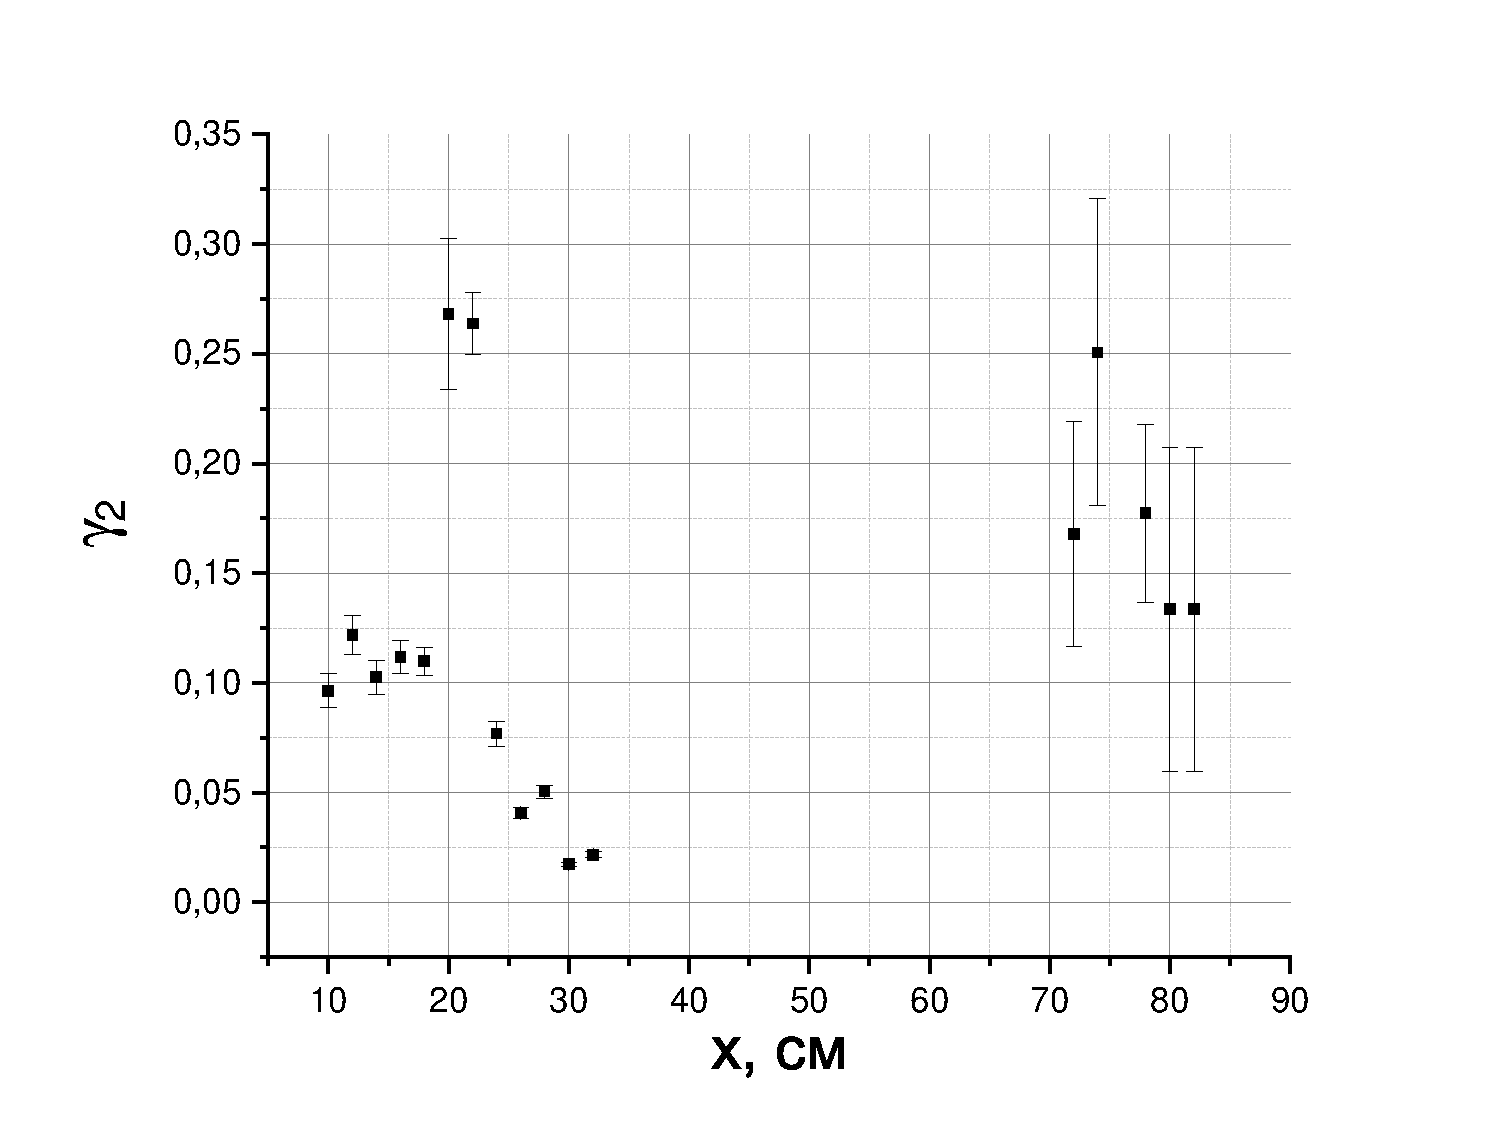
\includegraphics[scale=0.6]{graph2}
	\label{fig:graph2}
	\caption{График зависимости $\gamma_2(x)$}
	\end{center}
\end{figure}

\newpage

Из графика видно, что для двух последовательных максимумов: $x_1 = 20 \pm 2 \ см$ $x_2 = 74 \pm 2 \ см$. Определим расстояние L между зеркалами оптического резонатора лазера и межмодовое расстояние $\Delta \nu$

$$
L = \frac{1}{2} (x_2 - x_1) = 27 \pm 3 см
$$

$$
\Delta \nu = \frac{c}{2L} \approx = (5,6 \pm 0,6) \times 10^8 \ Гц
$$

Из графика: $l_{1/2} = 5 см$.Определим диапазон частот $\Delta F$ и оценим число генерируемых мод:

$$
\Delta F = \frac{0,26c}{l_{1/2}} \approx 1,6 \times 10^9 \ Гц
$$

$$
N = 1 + \frac{2 \Delta F}{\Delta \nu} \approx 6
$$

\section*{Выводы}

1.Из Рис 3 следует, что в пределах погрешности выполняется приближение $\gamma_3 = \cos^2(\alpha)$. Следовательно, поляризация хаотически меняется в пределах от 0 до $\pi$	
\\
2.Было получено значение расстояния между зеркалами резонатора лазера $L = 27 \pm 3 см$, которое более чем в 2 раза отличается от теоретического $L = 65 см$. Это может быть вызвано неточным исследованием зависимости $\gamma_2(x)$

\end{document}
